\part{Bloque 2}

Una vez implementado el comportamiento basado  en el movimiento de unidades se pasará a implementar distintos comportamientos propios de una IA táctica dentro de un entorno de juego de guerra en tiempo real.  En este bloque se hará un repaso por los distintos pasos y decisiones tomadas para superar los distintos apartados (Obligatorios y Opcionales) necesarios para implementar estos elementos.

Para esta práctica se utilizará todo lo implementado en la primera parte de la asignatura relacionado con movimiento de personajes, formaciones y colisiones.

El sistema de combate implementado consta de distintos tipos de unidades y terrenos, donde cada unidad tendrá distintos valores tanto de vida, ataque, alcance (Cuerpo a cuerpo y a distancia) y velocidad de movimiento que dependerá en muchos caso del terreno por el que se mueve el personaje. El mapa se ha implementado de forma manual como un grid, teniendo dos tipos de mapas. Por un lado el mapa convencional que consta de distintos tipos de terrenos, puntos de interés, bases, personajes,etc. Y por otro lado un mapa que mostrará las distintas influencias en forma de 'mapa de calor'.
\textbf{**COMENTAR ESTADOS**}
Además  existirán distintas zonas de interés táctico en el mapa como pueden ser puntos de curación, zonas de paso entre 'paises', bases o puntos intermedios de cruces de caminos. Cada una de estas zonas de interés tendrá un tipo de comportamiento dependiendo del equipo, por ejemplo, las bases solo podrán ser tomadas por personajes enemigos.

El movimiento de los personajes del juego estará condicionado por dos factores que se verán en las siguientes secciones. Por un lado tenemos el tipo de  terreno y por otro el tipo de personaje, y será la interacción de los distintos personajes con los distintos tipos de terrenos lo que marque el comportamiento y el valor de atributos como la velocidad en nuestros personajes.

\section{Interfaz gráfica}
El juego como ya se ha comentado consistirá en ver cómo los npcs aplican una estrategia concreta, en este caso es el jugador el que a través de botones puede interaccionar para cambiar la estrategia. En la siguiente figura podemos ver como queda la interfaz
\begin{figure}[H]
    \centering
    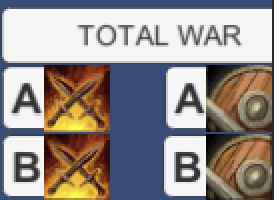
\includegraphics{buttons.png}
    \caption{Interfaz gráfica estrategia}
    \label{fig:mainButtons}
\end{figure}
Los iconos de espadas permitirán poner el modo ofensivo al equipo que se desee mientras que el icono del escudo permite indicar al equipo que se ponga a defender. El botón de \textit{Total war} cambia el comportamiento de todas las unidades del juego para que estas den prioridad al enfrentamiento y toma de la base rival. El juego comenzará con los botones desactivados.

\section{Campo de batalla}
En esta sección veremos los tipos de terrenos que se han utilizado, cómo se han usado y cual será su forma de afectar al movimiento de los personajes. El mapa de juego se ha creado en forma de \textit{grid} donde cada celda del \textit{grid} tendrá una etiqueta de tipo \textit{Floor} y una textura que permita distinguir el tipo de terreno. En total se han utilizado 10 tipos distintos de terrenos:
\begin{enumerate}
    \item Piedra gris: La piedra gris permite tanto delimitar los bordes de las bases como los pasos entre zonas. Es un material por el que a priori los personajes no tienen mayor dificultad para andar, exceptuando las unidades con montura que pueden resbalar en el por lo que deberían reducir su velocidad.  
    \item Camino marrón claro y marrón oscuro: Estos dos materiales son usados para crear calzadas por las que las unidades terrestres gustan andar y a priori todas podrán andar por estos caminos teniendo en cuenta que unas tendrán preferencia por el marrón y otras por el marrón claro. Las preferencias de movimiento se verán más adelante.
    \item Pradera: Es una zona en donde las unidades pesadas encontrarán dificultad para moverse, pero otro tipo de unidades más ligeras, en especial las unidades a distancia encontrarán facilidad de movimiento y sitio para atacar a unidades que puedan encontrarse en los caminos.
    \item Arena clara y oscura: Estas texturas formarán zonas de dunas de arena en donde la mayoría de unidades verán reducido su movimiento pero tendrán que atravesar si quieren conseguir algún sub-objetivo o zona de curación. 
    \item Agua: Las zonas de agua oscura serán las más profundas y que ninguna unidad será capaz de atravesar. Sin embargo, el agua más clara y menos profunda puede ser atravesada por unidades montadas o unidades ligeras, ya que las más pesadas pueden ser susceptibles de hundirse aquí.
    \item Suelo: Las zonas de suelo ajedrezadas indicarán donde se situan las bases  
    \item Lava: TBD
\end{enumerate}
El terreno de juego como podemos ver en **\textbf{INSERTAR FIGURA TERRENO TBD**} está formado por un grid de 52x52 donde se han representado 2 bases, la del equipo A en la zona inferior y el equipo B en la zona superior. Estas bases están separadas por un río que no se puede cruzar y conectadas por 3 puentes. Cada base está conectada por una serie de caminos hacia la base enemiga, encontrándose zonas de interés como zonas de curación.
\section{Tipos de Unidades}
Al habernos basado en un juego de captura de bases tipo RTS lo suyo era tener varias unidades que tengan movimientos variados dependiendo del terreno y de los personajes que se encuentren para pelear. Es por esto que se han implementando 4 tipos de unidades:
Unidades de infantería, unidad a caballo, Unidad Arquera y Unidad Lancera. Para distinguir las unidades se han usado unos assets de la store de unity .
\footnote{Toon RTS Units 3D \url{https://assetstore.unity.com/packages/3d/characters/toon-rts-units-67948}.}

Por cada unidad tendremos una clase distinta que hereda de la clase AgentNPC. Esta clase padre definirá una estructura de tipo diccionario $<$Terreno, Float$>$ donde a cada tipo de terreno se le asignará un multiplicador de velocidad para cada personaje, además esta clase definirá todos los atributos de un personaje como pueden ser la vida, velocidad de movimiento, ataque, etc.

Las clases hijas asignarán valores a estos atributos en función de las características que se les quieran asignar. Además tenemos el método \textit{generateDict} en cada clase de unidad, que será llamado en el awaka, donde se asigna a cada tipo de terreno un multiplicador de coste de movimiento para ese personaje, veamos como quedaría en el caso de la Unidad Lancero:
\begin{lstlisting}

private Dictionary<TerrainType, float> GenerateDict()
    {
        _costes.Add(TerrainType.GreyStones, 1f);
        _costes.Add(TerrainType.BrownStony, 0.75f);
        _costes.Add(TerrainType.BrownStonyLight, 0.5f);
        _costes.Add(TerrainType.SandyOrange,2.2f);
        _costes.Add(TerrainType.Sandy, 2f);
        _costes.Add(TerrainType.WaterLightBlue, 3f);
        _costes.Add(TerrainType.WaterDeepBlue, Mathf.Infinity);
        _costes.Add(TerrainType.Floor, 0.1f);
        _costes.Add(TerrainType.Lava, 5f);
        _costes.Add(TerrainType.Grass, 0.3f);
        return null;
    } \end{lstlisting}
    
En el método update de la clase AgentNpc antes de aplicar los steerings se recalculará la velocidad de movimiento en función del terreno   sobre el que esté el personaje:
\begin{lstlisting}
 public new void Update()
    {
        String textureName;
        base.Update();
        Ray NpcPos = Camera.main.ScreenPointToRay(Position);
        RaycastHit hitInfo;
        if (Physics.Raycast(NpcPos, out hitInfo) && hitInfo.collider != null)
        {

            if (hitInfo.collider.CompareTag("Floor"))
            {
             textureName = hitInfo.collider.gameObject.GetComponent<MeshRenderer>().material.mainTexture.name;
            _maxSpeed = _maxSpeed / _costes[getTerreno(textureName)];

            }
        }
        ApplySteering();
    }
\end{lstlisting}

El método \textit{getTerreno} simplemente devolverá el tipo de terreno en función del nombre de la textura detectada.\\

En la siguiente tabla podemos ver una relación de los tipos de unidades y su multiplicador de velocidad según el terreno. También veremos otra tabla con los distintos valores de influencia dependiendo del terreno y la unidad.
++INCLUIR TABLA VELOCIDADEES **

**INCLUIR TABLA INFLUENCIAS**


\section{Comportamiento táctico}

\begin{table}[H]
    \centering
    \begin{tabular}{|c|c|c|c|c|}
        \cline{2-5}        
        \multicolumn{1}{c|}{} & 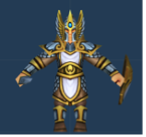
\includegraphics{imagesTable/infanteria} & 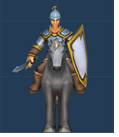
\includegraphics{imagesTable/caballo} & 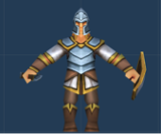
\includegraphics{imagesTable/lancero} & 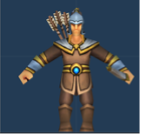
\includegraphics{imagesTable/arquero} \\
        \hline
        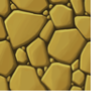
\includegraphics{imagesTable/claroPiedra} 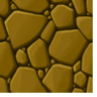
\includegraphics{imagesTable/piedra} 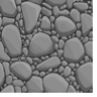
\includegraphics{imagesTable/grisPiedra} & 75\% & 75\% & 90\% & 90\% \\
        \hline
        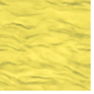
\includegraphics{imagesTable/arena} 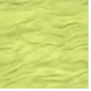
\includegraphics{imagesTable/claroArena} & 25\% & 25\% & 60\% & 60\% \\
        \hline
        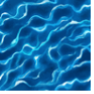
\includegraphics{imagesTable/agua} 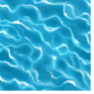
\includegraphics{imagesTable/claroAgua} & 0\% & 0\% & 0\% & 0\% \\
        \hline
        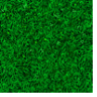
\includegraphics{imagesTable/hierba} & 50\% & 100\% & 45\% & 100\% \\
        \hline
        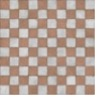
\includegraphics{imagesTable/suelo} & 100\% & 50\% & 100\% & 100\% \\
        \hline
        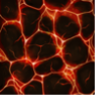
\includegraphics{imagesTable/lava} & 5\% & 5\% & 10\% & 2\% \\
        \hline
    \end{tabular}
\end{table}


\section{Mapa táctico}
En nuestro juego RTS se ha implementado un minimapa que nos permite tener en la esquina inferior derecha los distintos mapas de influencia y además la IA táctica se puede adaptar su comportamiento según esta influencia. En este apartado se verá los distintos mapas implementados y su influencia táctica.

\subsection{Mini mapas}
Utilizando un canvas de tamaño más pequeño se ha creado un panel en la esquina inferior derecha en donde se proyectarán diferentes texturas en tiempo real. Tenemos la cámara enfocada en nuestro terreno de juego principal y otra cámara enfocada en el terreno de las influencias y las texturas en tiempo real serán las que contendrán aquello que renderice la cámara. 

Si \textbf{presionamos la tecla I} podemos hacer que el mapa principal pase al minimapa y así ver en grande los distintos mapas de influencias.  Además en esta vista tenemos un boton que nos permite cambiar entre 3 tipos de mapa: influencia, vulnerabilidad y tensión.
%%capturas
\subsection{Comportamiento táctico: Map de Influencia}
El mapa de influencia se basa en que los distintos npcs y puntos de interés del juego tienen una influencia distintos, y estas influencias afectarán de distinta forma al comportamiento que tendrán los agentes a partir de la información que reciban de su entorno. Esta información usada por el agente puede ser el tipo de terreno, los agentes que tiene cerca, puntos de curación, etc. Este comportamiento influirá en donde se dirigen los personajes a la hora de atacar y defender. \\

El mapa de influencia se representará como un mapa de calor de color Rojo y Azul para los equipos A y B respectivamente. La influencia mostrada en el mapa se calculará como el agregado de las influencias que emite cada personaje.
%Cómo se calcula la influencia.

Esta información de influencias será usada como información táctica a la hora de calcular el comportamiento táctico de los personajes